
\section{Object Reconstruction}
\label{sec:cmsexperiment:reconstruction}

The layer structure of CMS detector, tracking-ECAL-HCAL-Muon, is idea to particle flow reconstruction, which uses information from all subdetector systems and reconstruct each final state particles, including muon, egamma and hadrons. Based on the particle flow candidates, jets met are computed and BTag and hadronic tau are identified in the jet collections. 

Fig~\ref{fig:cmsexperiment:reconstruction:pfa} illustrates the function of the sub detector and how different final state particles behave in them. Starting from the beam interaction region, particles first enter a tracker, in which charged-particle trajectories (tracks) and origins (vertices) are reconstructed from signals (hits) in the sensitive layers. The tracker is immersed in a magnetic field that bends the trajectories and allows the electric charges and momenta of charged particles to be measured. Electrons and photons are then absorbed in an electromagnetic calorimeter (ECAL). The corresponding electromagnetic showers are detected as clusters of energy recorded in neighbouring cells, from which the energy and direction of the particles can be determined. Charged and neutral hadrons may initiate a hadronic shower in the ECAL as well, which is subsequently fully absorbed in the hadron calorimeter (HCAL). The corresponding clusters are used to estimate their energies and directions. Muons and neutrinos traverse the calorimeters with little or no interactions. While neutrinos escape undetected, muons produce hits in additional tracking layers called muon detectors, located outside the calorimeters. As a result,  muons leaves tracks in the tracker and muon chamber with MIP in ECAL and HCAL. Electrons and phontons deposit energy in the ECAL with and without track correspondence respectively. Charged and neutral hadrons deposit energy in both ECAL and HCAL with and without track correspondence respectively. 

\begin{figure}[ht]
    \centering
    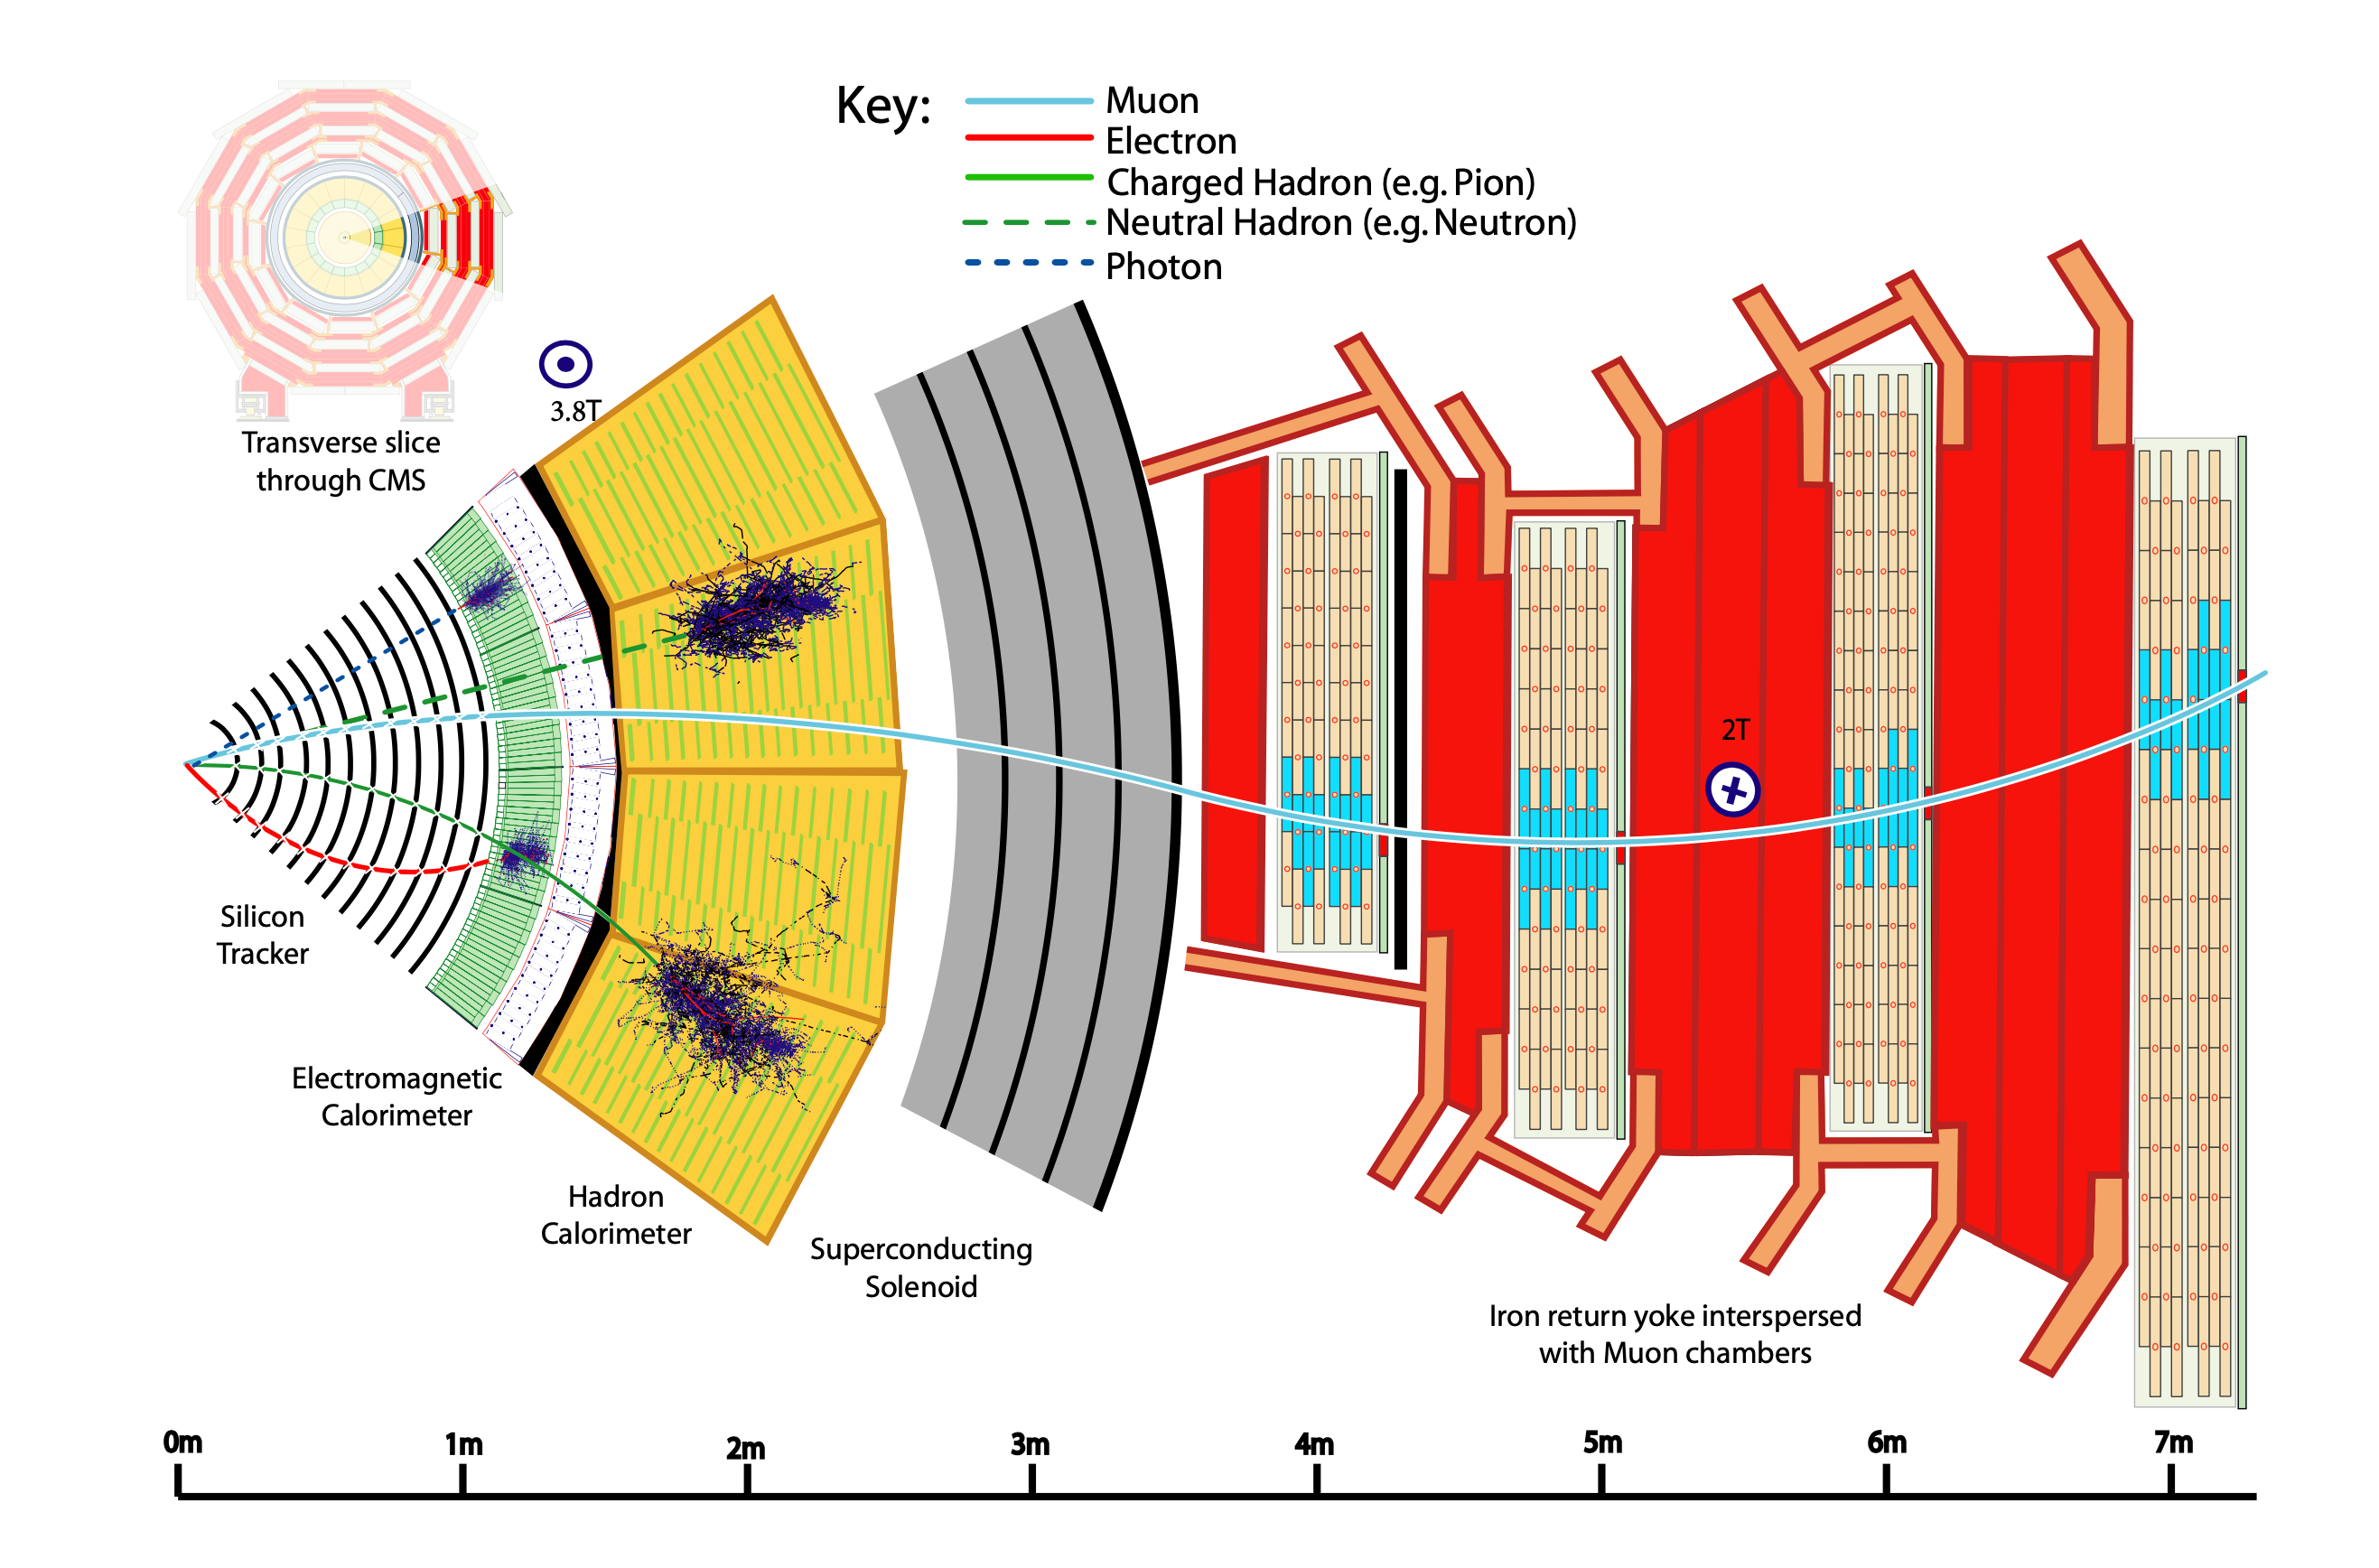
\includegraphics[width=0.8\textwidth]{chapters/CMSExperiment/sectionReconstruction/figures/pfa.png}
    \caption{Caption}
    \label{fig:cmsexperiment:reconstruction:pfa}
\end{figure}

The FPA begins with computing PF element in each subdetector: tracks in the tracker and muon chamber, clusters in ECAL and HCAL. Then PF elements in different subdetectors are linked to form PF Blocks via a linking process. PF Block summary the activity of potential particle candidate in each subdetector. The details of reconstruction of PF elements and their linking can be found in []. In the end, each PF blocks are identified into PF candidates, final state particles including muon, egamma and hadrons based on which JetMET, BTag and Tau ID are further computed.





\subsection{Muon}

The reconstruction of muon involves standalone reconstruction in the muon system, followed by globle muon reconstruction add trajectories in the tracker. The standalone reconstruction starts with the track segments in the individual muon chambers. The state vectors (track position, momentum, and direction) associated with the segments found in the innermost chambers are used to seed the muon trajectories, working from inside out, using the \acrfull{kf} technique \cite{tech:kf:Fruhwirth:1987fm}. The track parameters and the corresponding errors are updated at each step. The procedure is iterated until the outermost measurement surface of the muon system is reached. A backward Kalman-filter is then applied, working from outside in, and the track parameters are defined at the innermost muon station. Finally, the track is extrapolated to the nominal interaction point and a vertex-constrained fit to the track parameters is performed.

The global muon reconstruction consists in extending the muon trajectories to include hits in the silicon tracker. tarting from a standalone reconstructed muon, the muon trajectory is extrapolated from the innermost muon station to the outer tracker surface, taking into account the muon energy loss in the material and the effect of multiple scattering. This extrapolation and the associated uncertainty defines a region of interest in the tracker, where track candidates are seeded by hit doubles and reconstructed using Kalman-filter. A set of trajectory fits to the global hits are carried out to exact the muon momentum and impact parameters. This retain both prompt muons and muons from hadrons decays with the highest possible efficiency.

\begin{figure}[ht]
    \centering
    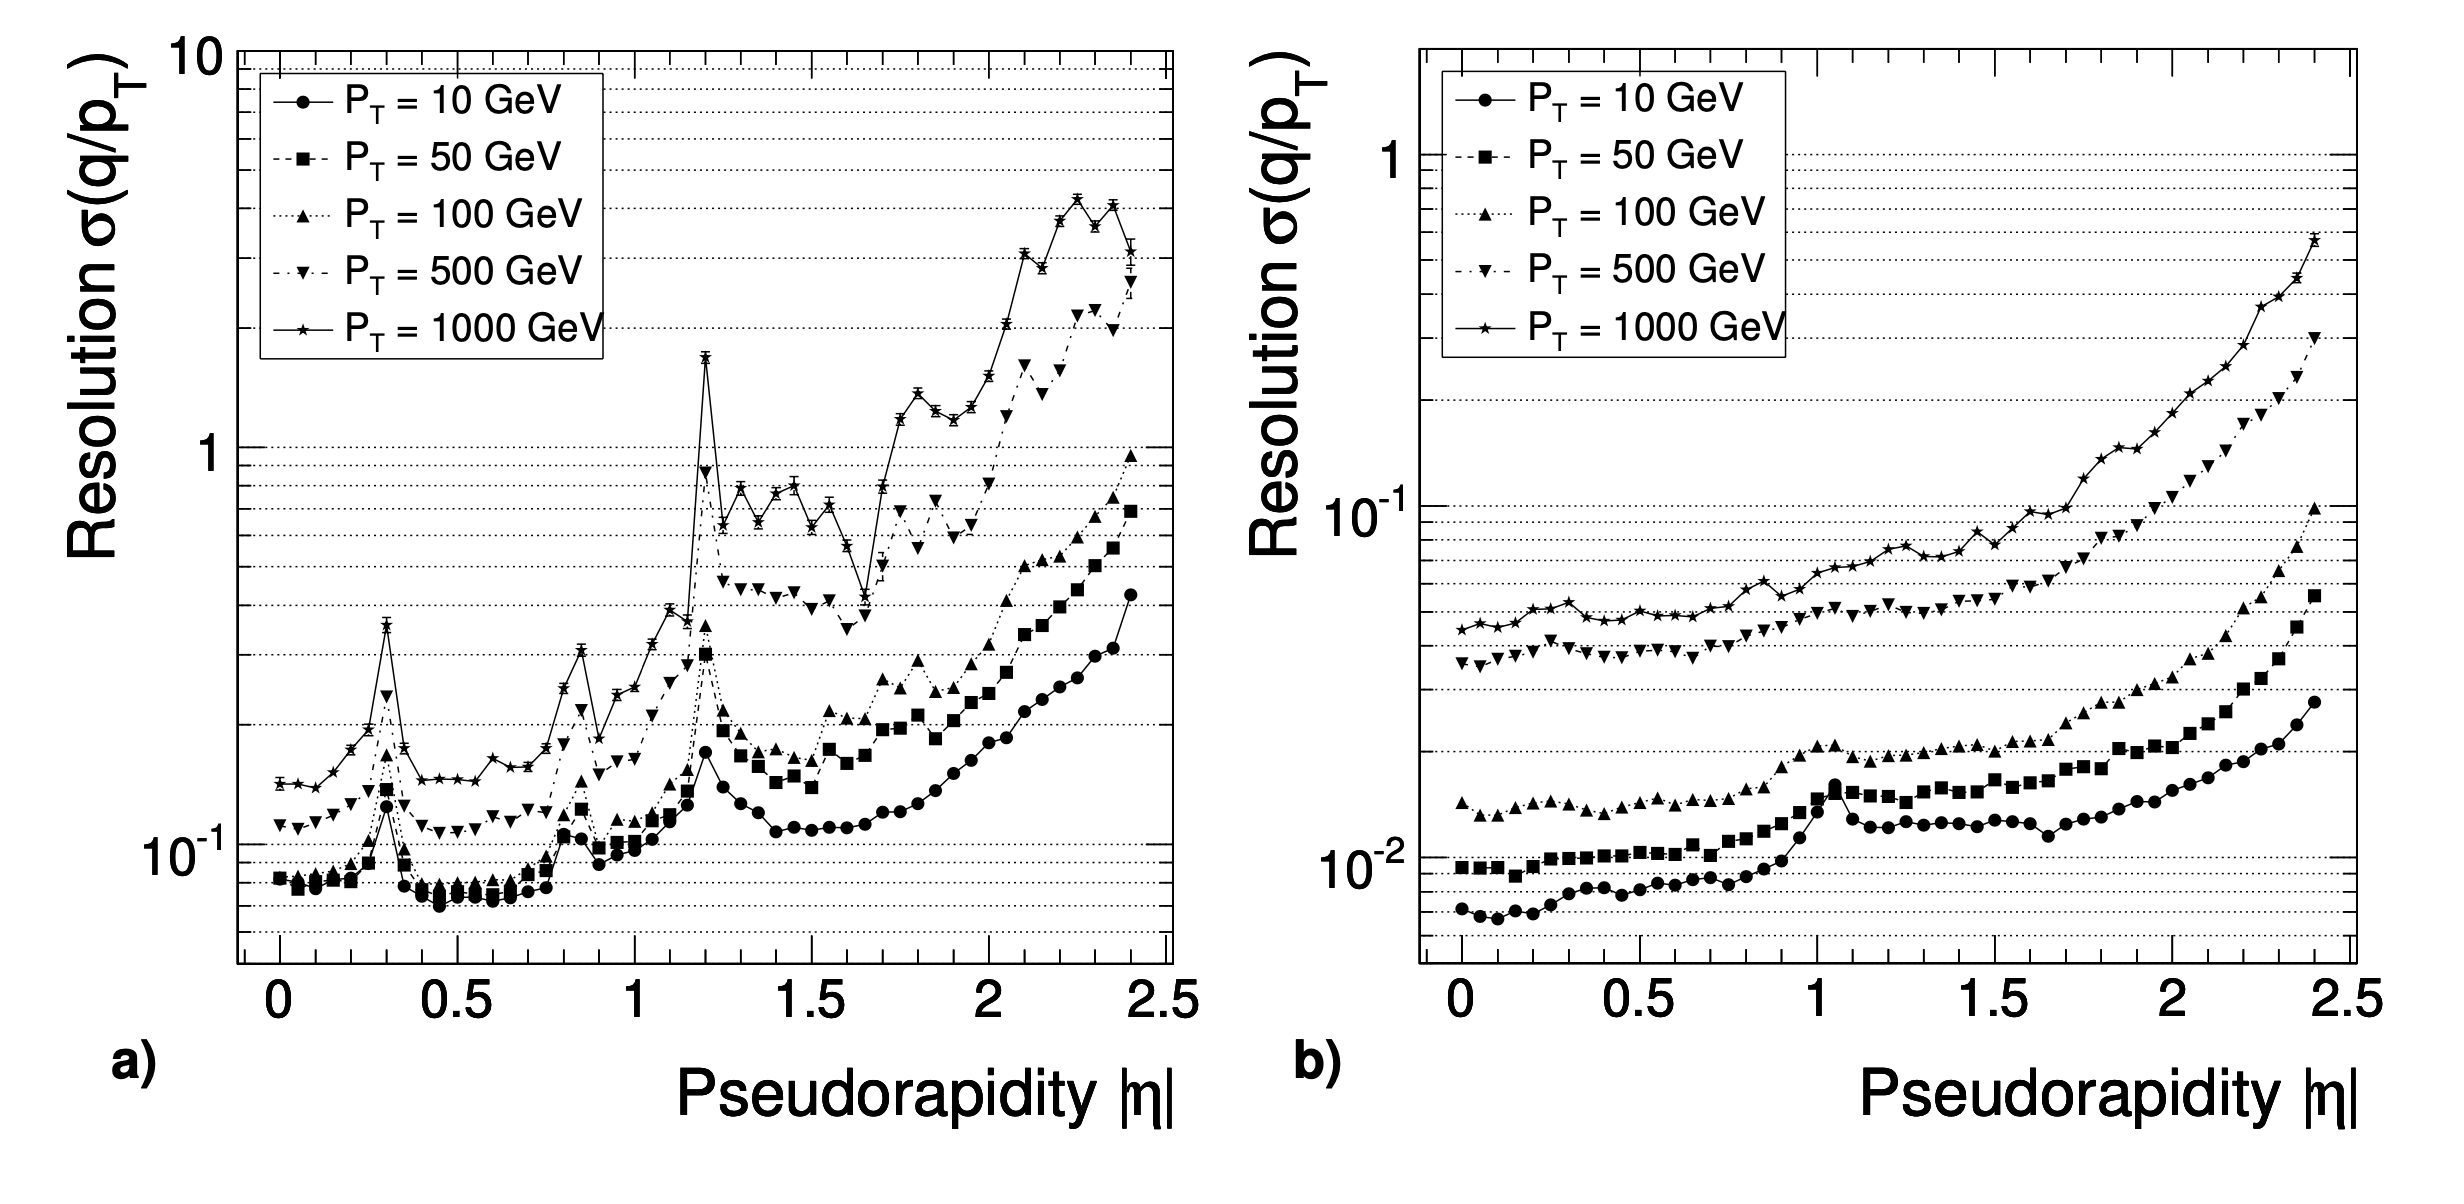
\includegraphics[width=0.95\textwidth]{chapters/CMSExperiment/sectionReconstruction/figures/resMu.png}
    \caption{Momentum resolution as a function of }
    \label{fig:cmsexperiment:reconstruction:resMu}
\end{figure}


Figure~\ref{fig:cmsexperiment:reconstruction:resMu} shows the transverse momentum resolution of muons with different energies for standalone reconstruction algorithm (a) and the global reconstruction algorithm (b). A significant improvement is achieved when going from standalone to global muon reconstruction.





\subsection{EGamma}

\begin{figure}[ht]
    \centering
    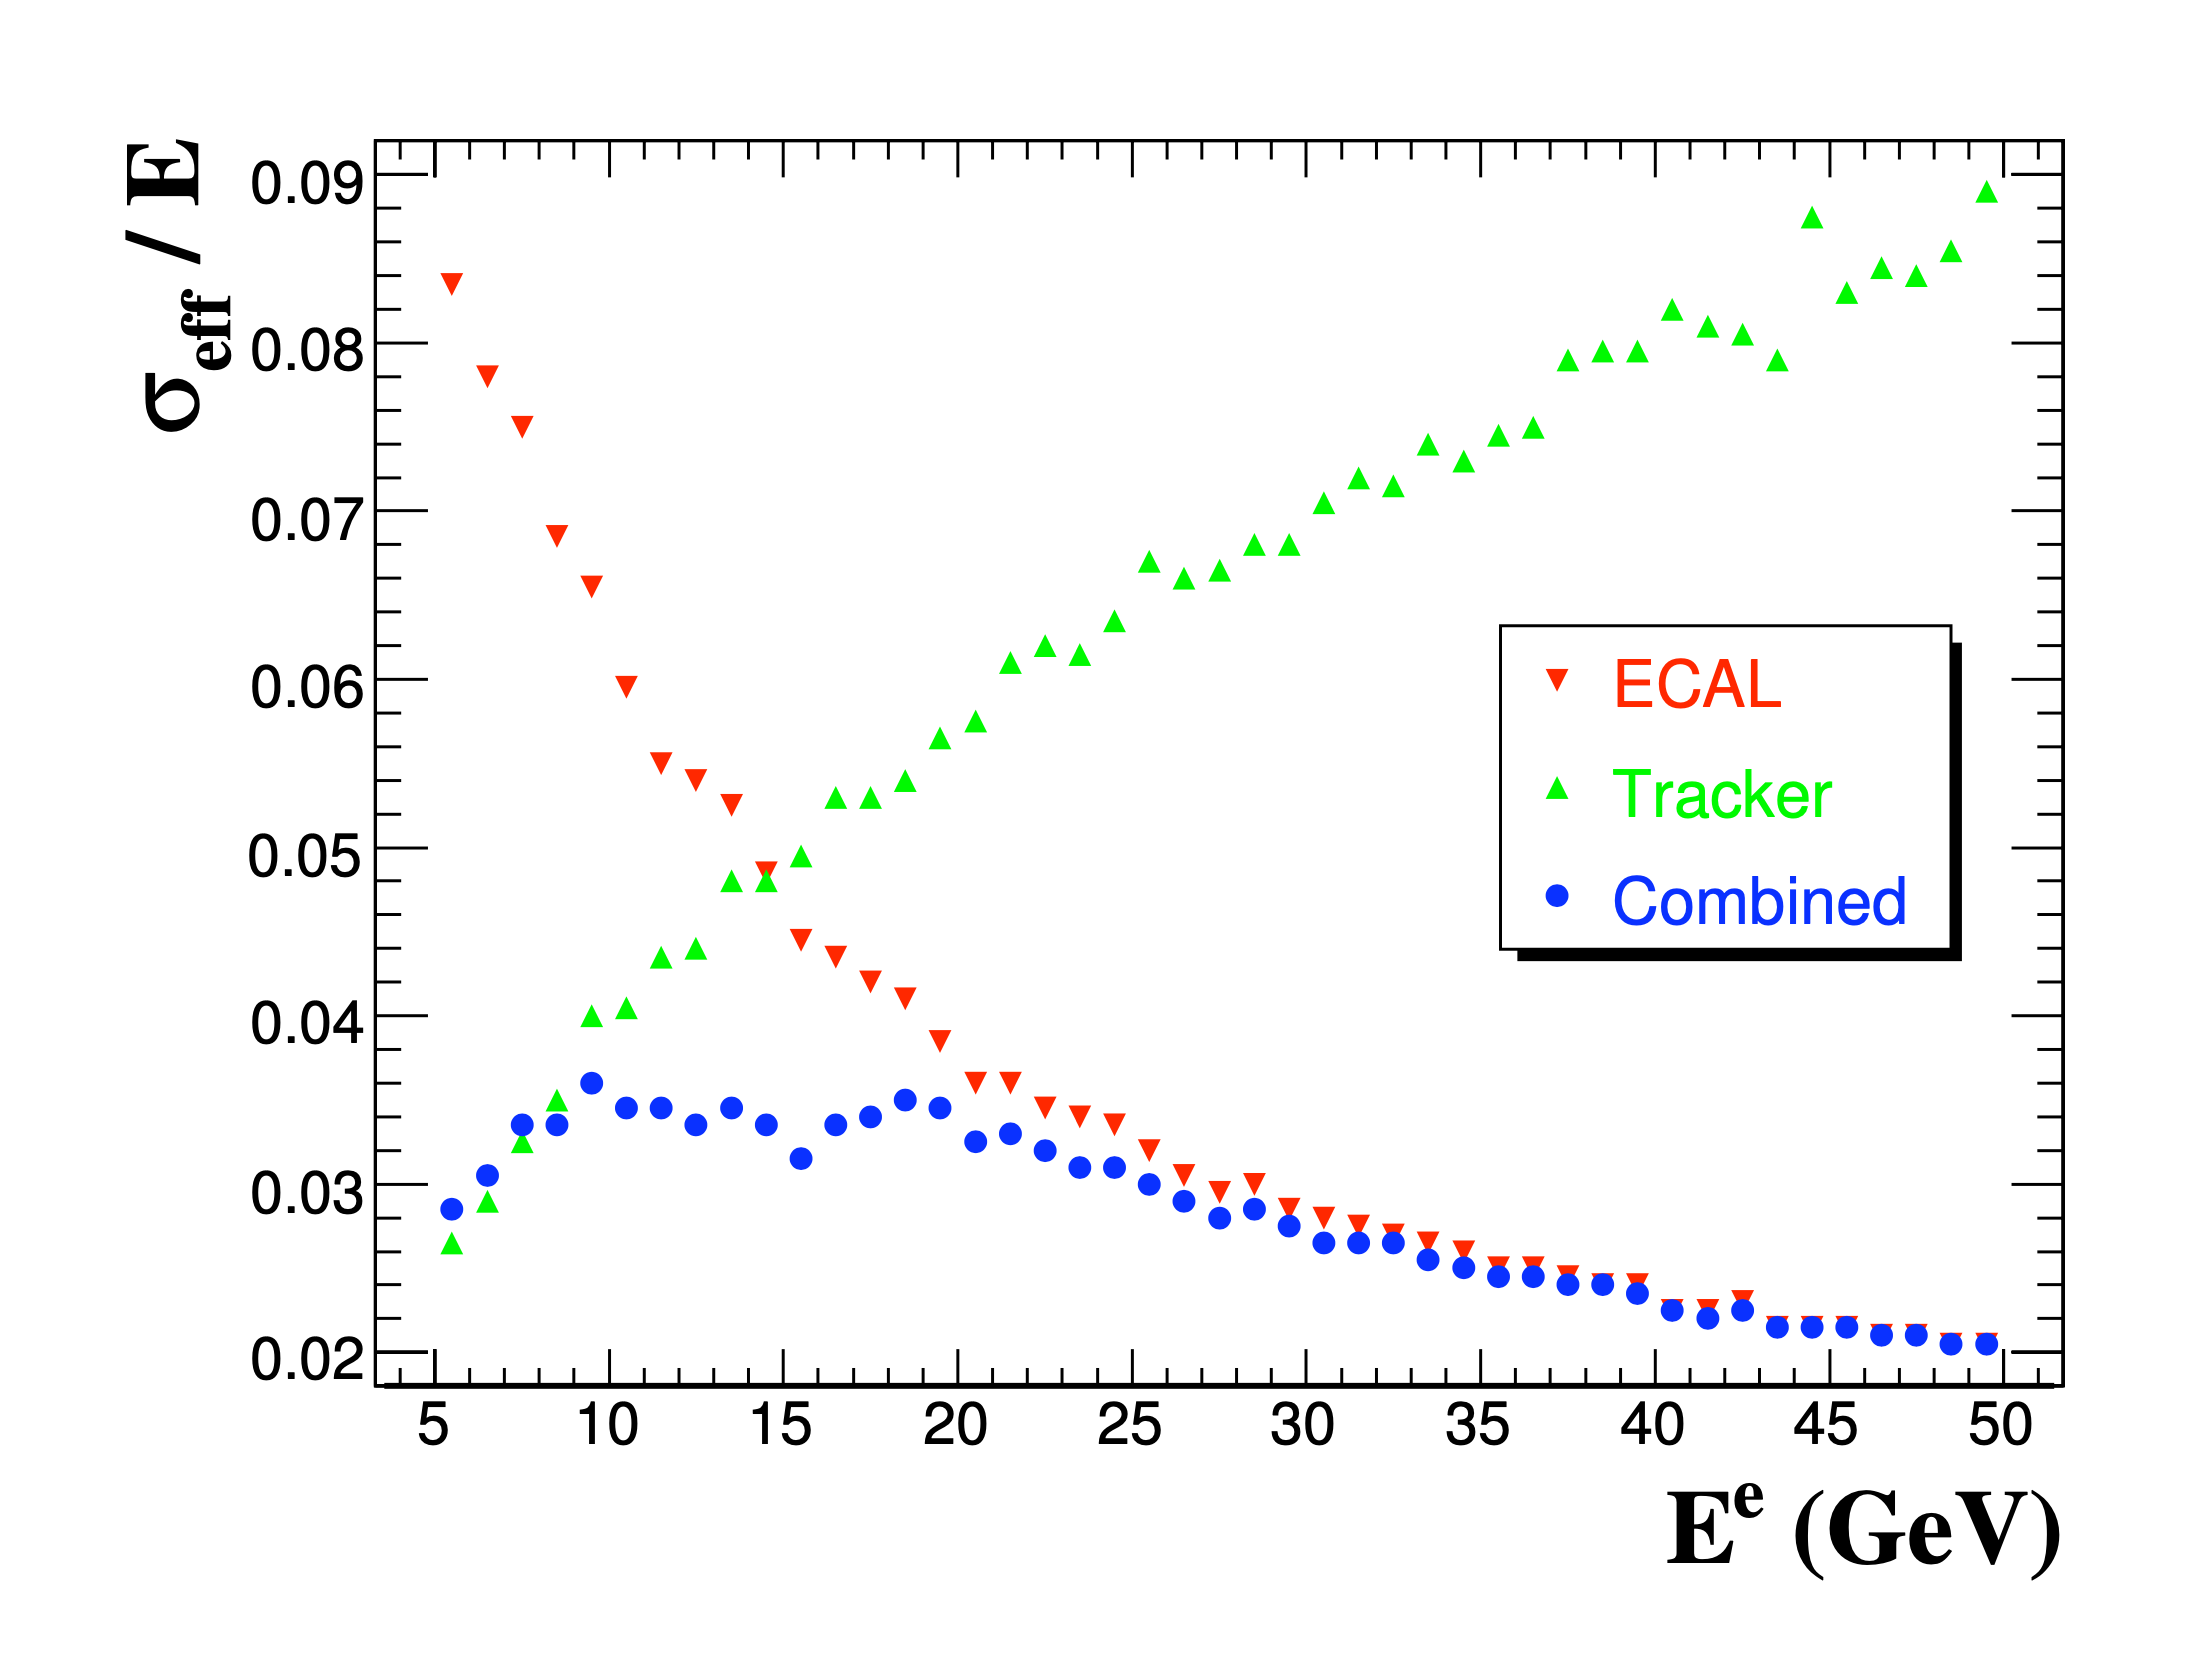
\includegraphics[width=0.5\textwidth]{chapters/CMSExperiment/sectionReconstruction/figures/resEle.png}
    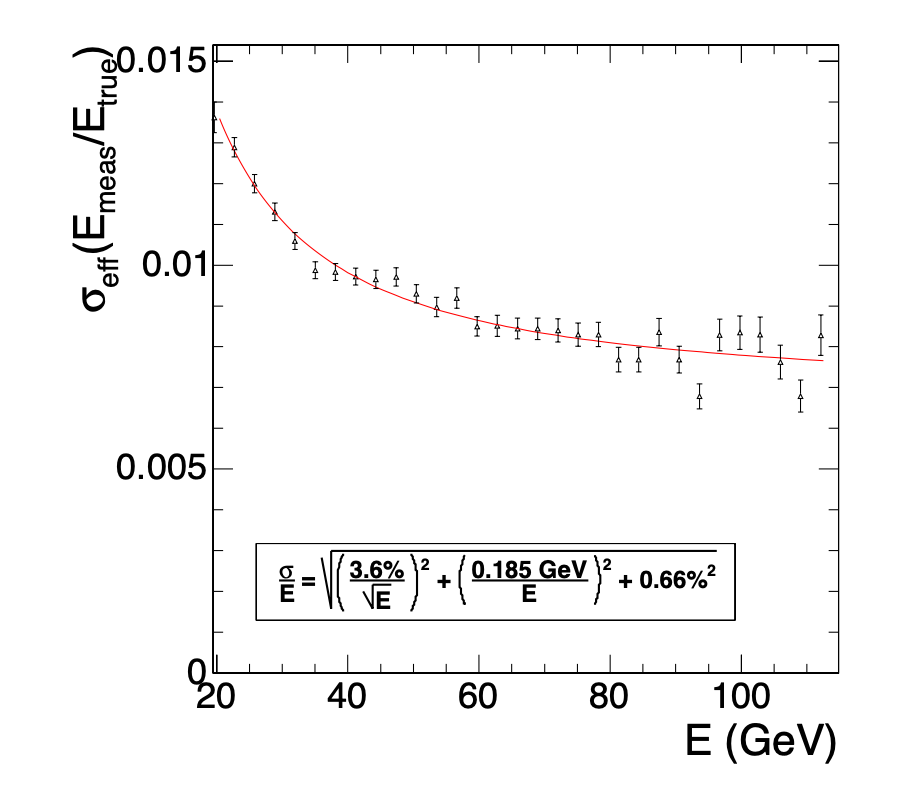
\includegraphics[width=0.42\textwidth]{chapters/CMSExperiment/sectionReconstruction/figures/resGamma.png}
    \caption{Caption}
    \label{fig:cmsexperiment:reconstruction:resEle}
\end{figure}

The electron reconstruction in CMS is hampered by the amount of tracker material which is discretely distributed in front of the ECAL. The material thickness varies strongly with $\eta$, raising from 0.3 $\chi_0$ at the central barrel to 1.5 $\chi_0$ at the barrel edge, then falling to 0.7 $\chi_0$ in the endcap inner edge. When electrons traversing the silicon layers of the pixel and inner tracker detectors, they radiate collections of bremsstrahlung photons and the energy reaches the ECAL spread in $\phi$. \cite{cms:tdr1:Bayatian:2006nff} provides an good illustration -- ''For electrons at $p^T=$10 GeV, about half of the electrons radiate away more than half of their energy before reaching the surface of the ECAL. In about 10$\%$ of the cases, more than 95$\%$ of the initial electron energy is radiated!'' Further more, the radiated photon can convert into electron-positron pairs, which are usually soft and trapped in the field loosing all energy in the end undetected.

The reconstruction of electron start with making superclusters of ECAL energy deposits. The superclustering algorithm is optimized for the scenarios of energy spread in $\phi$. The supercluster drives the finding of track seeds, which is hit doublets in pixel. If a seed compatible with the supercluster is found, tracks building begins inside-out with a nonlinear filter approach called \acrfull{gsf} \cite{tech:gsf:Adam:2005bya}. For supercluster linked with GFS tracks by particle-flow algorithm, an electron candidate is made and a fit to the GSF track and ECAL superclusters is used to extract the four-momentum measurement under the electron assumption. This not only provides combines the advantages of trackers in low energy region and the ECAL in the high energy region, but also connect the low energy and high energy region smoothly. The energy resolution of electrons using tracker, ECAL and combined is shown in Figure~\ref{fig:cmsexperiment:reconstruction:resEle} left. For supercluster not linked to GFS tracks, an photon candidate is made and the energy is obtained from the sum of energy deposited in a supercluster of crystals. To quantify the lateral spread of photon shower, a variable R9 is defined as the ratio of sum energy in 3x3 crystals around the highest crystal and the total energy sum in the supercluster. Energy resolution of photons with R9 >0.943 is shown in Figure~\ref{fig:cmsexperiment:reconstruction:resEle} right.



\subsection{hadrons}
Once muons, electrons, and isolated photons are identified and removed from the PF blocks, the remaining particles to be identified are hadrons from jet fragmentation and hadronization. These particles may be detected as charged hadrons and neutral hadrons, among which $\pi^0$ decays to two non-isolated photons. The ECAL and HCAL clusters not linked to any track give rise to non-isolated photons and neutral hadrons. Within the tracker acceptance ($|\eta|< 2.5$), all these ECAL clusters are turned into non-isolated photons and all these HCAL clusters are turned into neutral hadrons. 

Charge hadrons are made from the remaining calorimeter clusters and tracks. Each of the remaining HCAL clusters of the PF block is linked to one or several tracks and these tracks may in turn be linked to some of the remaining ECAL clusters. It is possible that calorimeter clusters also include unresolved FSR photons or close-by non-isolated neutral hadrons around charged hadrons. To identify unresolved neutral components around charged hadron, a match of calibrated calorimeter energy and tracker momentum is carried out. If the calibrated calorimetric energy is compatible with the sum of the track momenta, no neutral particle is identified. The charged-hadron momenta are redefined by further calibration taking into account information from both tracker and calorimeter. If the calibrated calorimetric energy is in excess of the sum of the track momenta by an amount larger than the expected calorimetric energy resolution for hadrons, the excess may be interpreted as the presence of photons and neutral hadrons. The excess energy is first treated as a non-isolated photon and subtracted from the ECAL energy. If ECAL energy alone is not enough to account for the excess, the remaining excess is treated as a neutral hadron. If the calibrated calorimeter energy is smaller than the tracking momentum, a search for non-isolated muon in the track projection is carried out with relaxed muon reconstruction standard and momentum of the reconstructed muons is subtracted before a re-compare.



\subsection{Jet and Met}

\begin{figure}[ht]
    \centering
    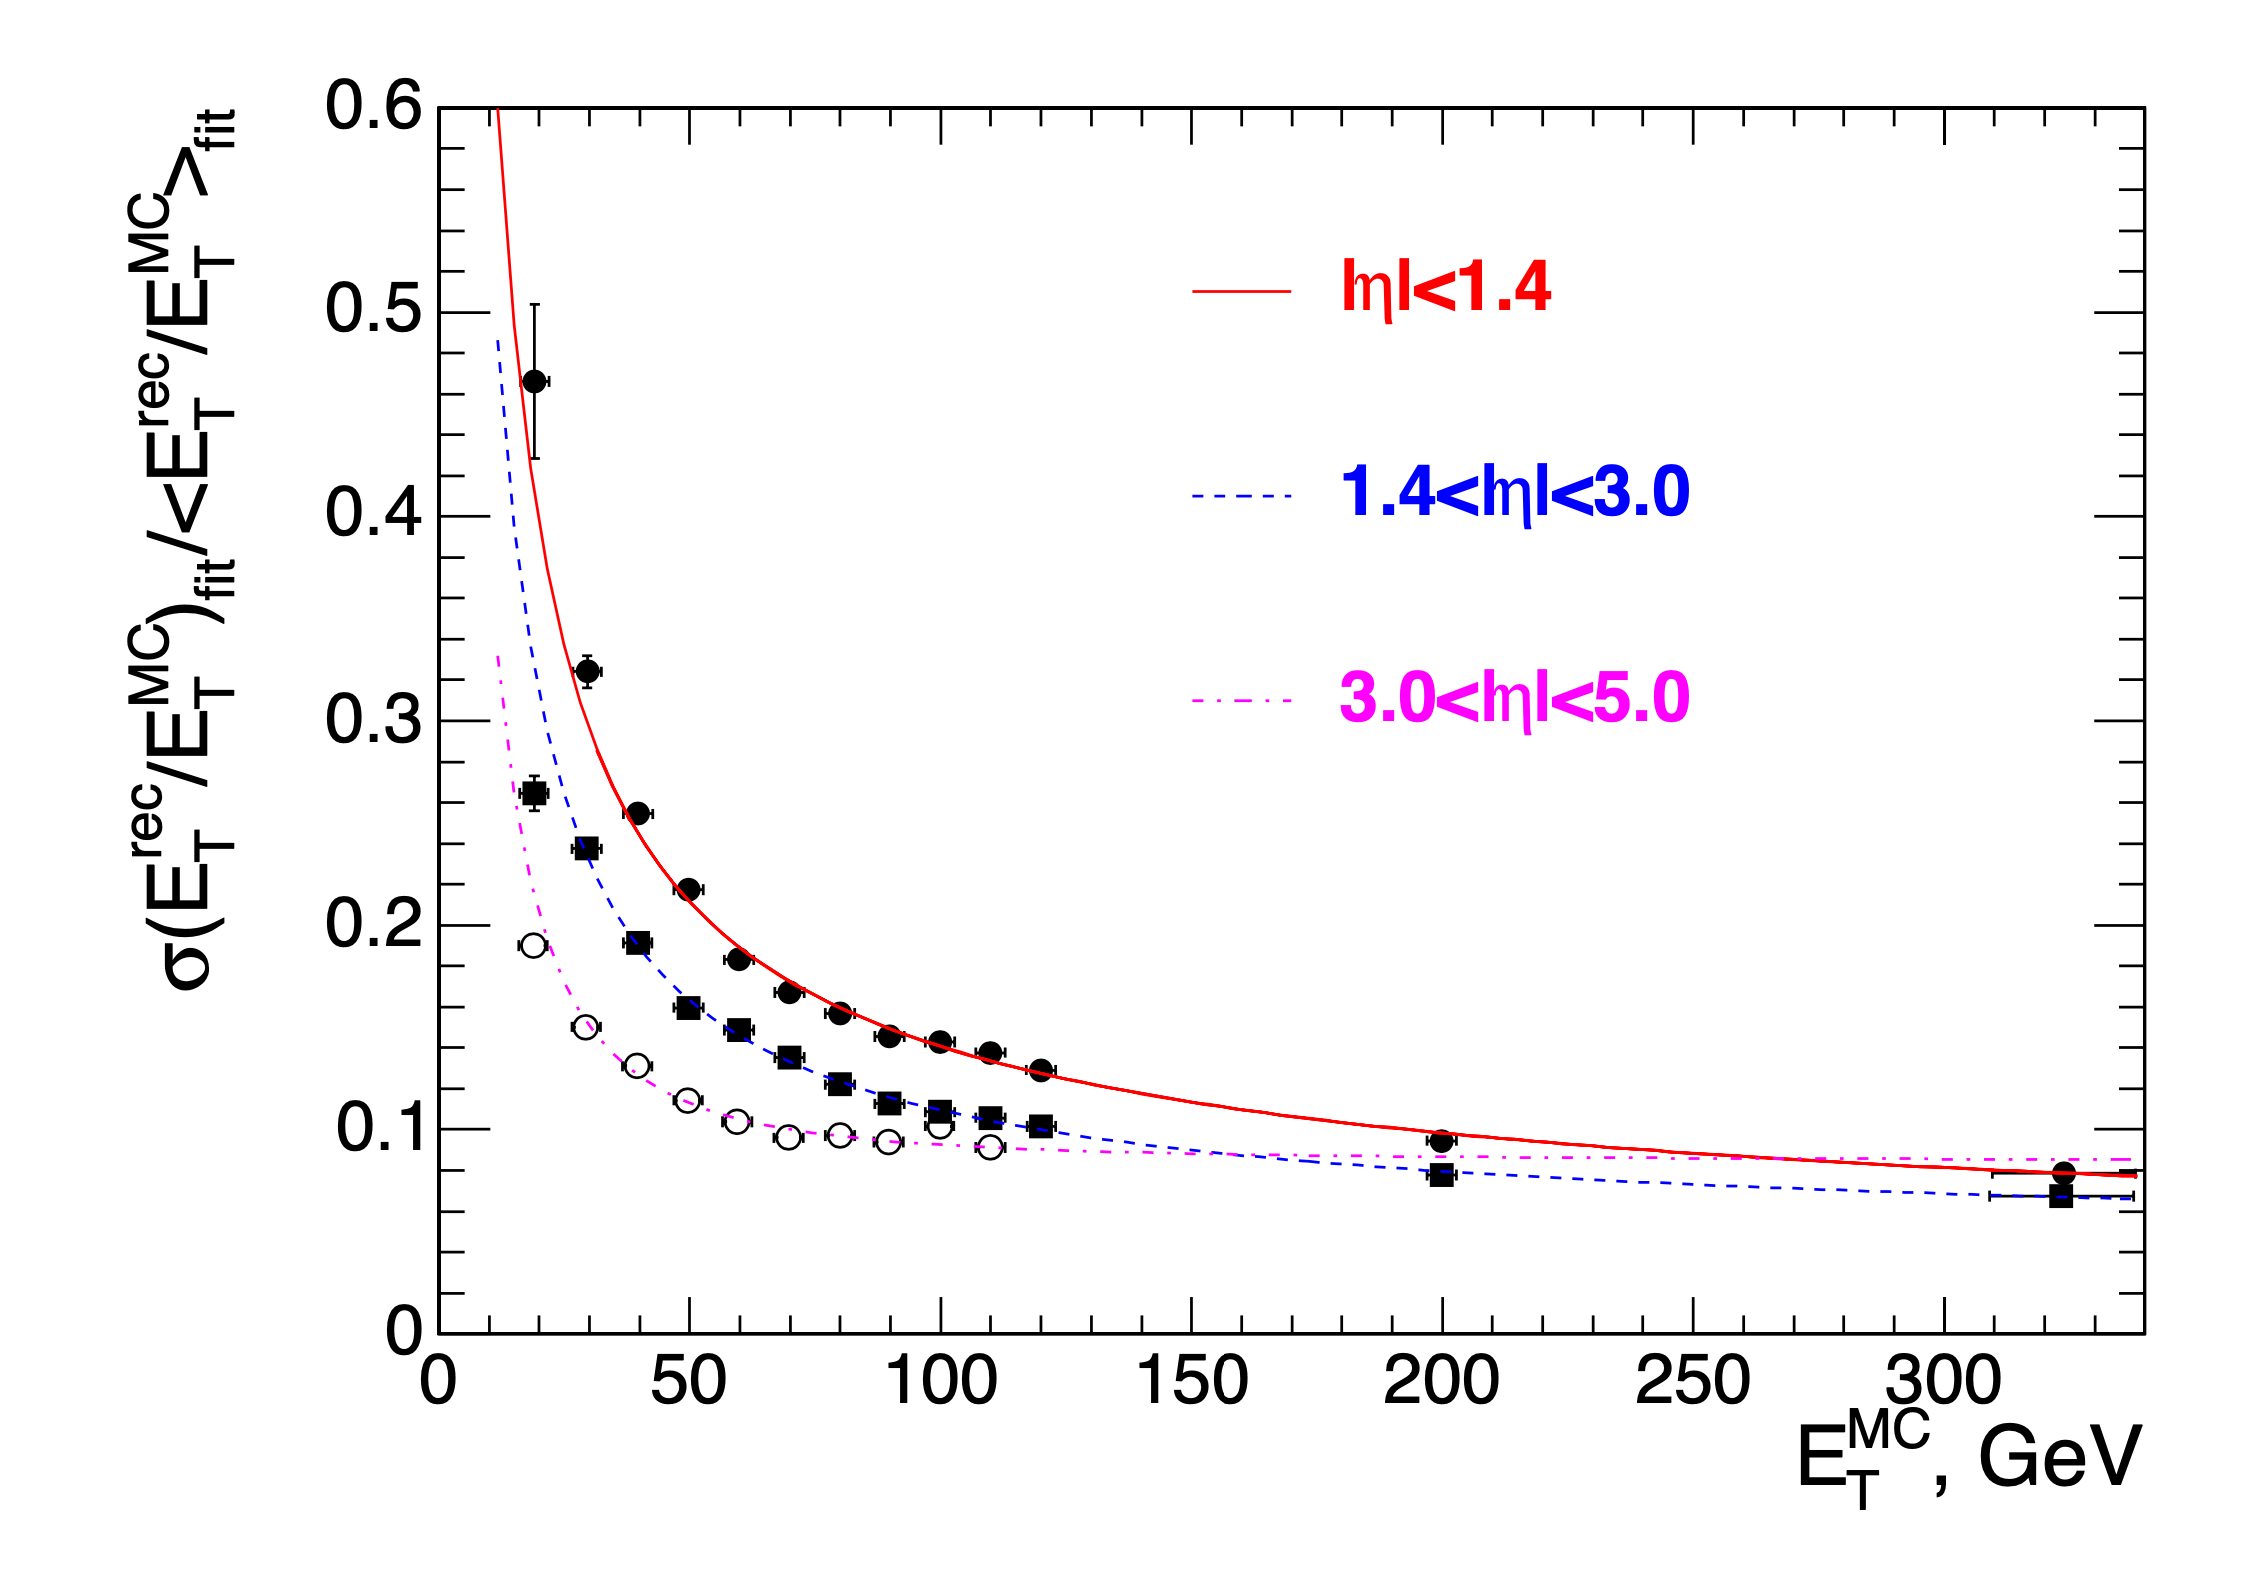
\includegraphics[width=0.6\textwidth]{chapters/CMSExperiment/sectionReconstruction/figures/resJet.png}
    \caption{Caption}
    \label{fig:cmsexperiment:reconstruction:resJet}
\end{figure}

Jet are reconstructed by clustering PF candidates using anti-kt algorithm \cite{tech:antikt:Cacciari:2008gp}. The energy resolution of jet is shown in Figure~\ref{fig:cmsexperiment:reconstruction:resJet}. Met is computed by balancing the total visible transverse momentum. 



\subsection{bTagging}
Jets originated from heavy flavor quarks are tag via multi-variational method taking into account the displacement of secondary vertices.

\subsection{Tau ID}
 Jets originated from hadonic taus are tagged via iso-plus-striped algorithms.

